\documentclass[11pt]{article}
\usepackage[includeheadfoot, top=1.0in, bottom=1.0in, hmargin=1.0in]{geometry}
\usepackage[utf8]{inputenc}
\usepackage{fancyhdr}
\usepackage{url}
\pagestyle{fancy}
\usepackage{setspace}
\usepackage{tabularx}
\usepackage{graphicx}
\usepackage{caption}
\usepackage{subcaption}
\usepackage{hyperref}
\usepackage{multicol}
\usepackage{amsmath}
\usepackage{enumitem}

\usepackage{hyperref}
\hypersetup{
    colorlinks=true,
    linkcolor=blue,
    filecolor=magenta,      
    urlcolor=blue,
}


\lhead{Astronomy Lab II}
\rhead{Spring 2023}
\lfoot{Sullivan \& Cassese}
\rfoot{Tues 7-10pm}
\cfoot{\thepage}

\begin{document}

\begin{center}
\huge{Lab 10: Indoors and Historical Observing}\\ \medskip \Large{April 11, 2023}
\end{center}

Hello! Today was supposed to involving observing outside with telescopes, but unfortunately it's too cloudy for that. Instead, we'll go through three related indoor activities. First, we'll start with a mini-lecture about modern observations and look at some data collected earlier this year in Arizona. After that we'll look at some images taken during one of the earliest research-grade photographic surveys, then finally we'll characterize some small telescopes using standard charts.

\section{Introduction and Modern Observing}

After the mini lecture, answer the following:


\begin{enumerate}
    \item Briefly describe each of the following:
    \begin{itemize}
        \item Bias image
        \item Flat field
        \item Dark image
    \end{itemize}
    \item Why are modern detectors cooled down to very low temperatures?
    \item How are most color photographs of the night sky put together?
\end{enumerate}

\section{Historical Astronomy and the Palomar Sky Survey}

Before the invention of modern cameras and CCDs, going to observe involved exposing large photographic plates, developing them, then making prints. This was a difficult and tedious process: photographic plates are much less sensitive to light than modern CCDs, so astronomers would have to wait many hours for enough photons to strike their glass to make an imprint. Even harder, modern computers could not keep the telescope aimed automatically, so observers would have to personally ``guide by eye" all night, staying in the cold dome to make sure their image stayed centered.

\medskip \noindent
This is all almost charming to think about now, and the implications of physical data are increasingly fascinating the deeper you go. One challenge that we now take for granted in the era of automated pointing: if you want to observe something too faint to see with your eye through the telescope, how do you know you're pointing in the right place? Knowing the coordinates are one thing, but when you're physically looking down the barrel of the telescope, how do you know what you're looking at?

\medskip \noindent
To help alleviate this, the Palomar Sky Survey undertook the first ever full-sky photographic atlas, finishing in 1958. Using a wide field of view telescope in Southern California, researchers took photographs of every patch of available sky, then made prints of those photos and sold them to universities. So, if an astronomer wanted to look for a target at some coordinate, they could now go down to their library, find the Palomar Sky Survey image of that region of the sky, take a polaroid photo of that, and bring the snapshot to the mountain with them. This ``finding chart", or a snapshot of the brightest objects near their target, would let them line up the telescope in the right place to begin taking their own pictures.

\medskip \noindent
Columbia has a set of this survey: it's the cabinet in the corner of this room. We're going to look at some of the images, but please: \textbf{These prints are very difficult to replace. Please treat them gently and do not leave any food or drink near them. Do not write on the prints, or on the transparencies.}

\medskip \noindent
Complete all three sections, but feel free to do them in any order, and to collaborate. Note the following:
\begin{itemize}
    \item Each region of the sky was imaged at two wavelengths. The E plates were sensitive to red light and the O plates were sensitive to blue light
    \item The scale of these prints is inverted: dark regions on the plate correspond to bright regions on the sky, and vice versa
    \item The exposures of the two photographs (red and blue) were scaled such that a star with the same color as the sun will appear to have the same brightness on the two prints.
\end{itemize}

\subsection{PLATE +60, 23:28:00}
This plate show an emission nebula, or a region of massive star formation. In these regions, hot massive stars emit ultraviolet light which ionizes atoms in the clouds, causing them to emit a wavelength of light which corresponds to a specific spectral line of Hydrogen (called H$\alpha$).
\begin{enumerate}
\setcounter{enumi}{3}
    \item Give the coordinates of the brightest part of the nebula
    \item Is the nebula brighter on the blue or red plate?
\end{enumerate}

\subsection{PLATE +42 00:30:00}
This plate shows the nearest major galaxy to the Milky Way, Andromeda. I cannot find the E plate, or the transparency... which is frustrating. Still, consider this one image and answer the following:
\begin{enumerate}
\setcounter{enumi}{5}
    \item What do you notice about the shape of Andromeda, the structure?
    \item Which part of Andromeda is brighter, the center, or the edges?
    \item Look at the object just above Andromeda. What do you think this is?
\end{enumerate}

\subsection{PLATE +30, 09:32:00}
This is a fairly random patch of sky with not too many stars and not much else interesting going on. However, it's a good example of how stars look different when you view them in different wavelengths.
\begin{enumerate}
\setcounter{enumi}{8}
    \item Pick out the 5 brightest stars on the blue print. List their positions (RA and DEC) and give their ID number given on the transparency.
    \item Now find the same 5 stars on the red print. Indicate which stars appear brighter on the blue print, the red print, or if they have equal brightness on both prints.
    \item Which of the above stars are hotter than the Sun, about the same temperature as the Sun, or cooler than the Sun? How do you know this?
\end{enumerate}


\section{Indoor Observing}
(Adopted from David Schiminovich's Observing Lab). \\
Today, as a means of introduction, we’ll explore aspects of angular measurement on
astronomically important angular scales, from degrees (°) to arcminutes (‘) to arcseconds (“).
Specifically, we’ll focus on the field of view and angular resolution of astronomical instruments commonly used for naked eye observations, and think about implications for carrying out observations of astronomical objects.

\medskip \noindent
For all below, recall that 1° = 60’ = 3600”

\subsection*{Learning Goals}
By the end of this section you will have:
\begin{itemize}
    \item Developed some intuition for some angular scales and using your body to measure approximate angles
    \item Developed an intuition for the field of view and angular resolution of your eye and of several commonly used astronomical observing instruments (binoculars, telescopes), in some cases utilizing different eyepieces. You might also experiment with your phone camera
\end{itemize}

\begin{figure}[t!]
    \centering
    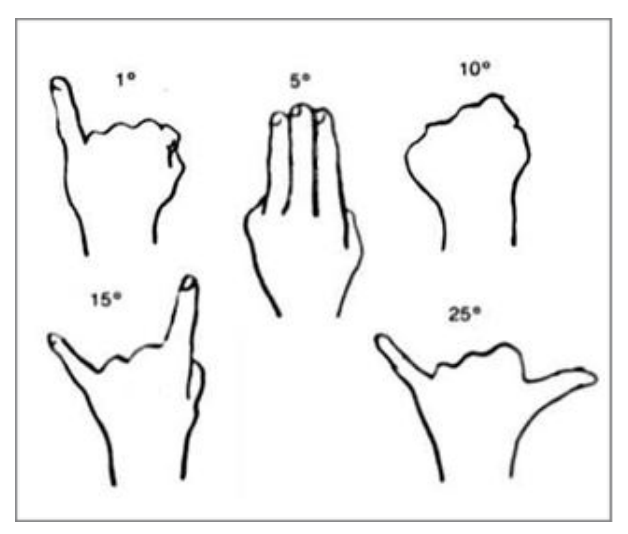
\includegraphics[width=.75\textwidth]{Images/AngSize.png}
    \caption{Angle measurements (from \url{http://oneminuteastronomer.com})}
    \label{fig:Hem}
\end{figure}

\subsection{Measuring approximate angles using your body}
Ultimately we’ll need a device that will help us use angular coordinates to locate objects in the sky, and measure angular separations between objects. Sometimes, even a coarse ability to make measurements on degree scales can be useful in situating yourself on the celestial sphere.

\medskip \noindent
For the questions below we will use our own bodies as protractors. Later in the lab we will measure angles more precisely using measured distances with a ruler or calibrated reference scale.

\medskip \noindent
We can use our hands as a measuring device by holding them at arm’s length. See Figure 1 for angular approximations that assumes our bodies scale similarly (e.g. people with longer arms
usually have larger hands than people with short arms)

\bigskip \noindent
\textbf{Validating your body angles:}

\medskip \noindent
Measure 1) the width (w) of your pinky, 2) the width (w) of your hand with thumb and pinky outstretched, and 3) the length of your arm (distance, d). Using trigonometry, estimate the angle subtended by your finger and hand at arm’s distance in degrees. You can approximate angle $\theta = \frac{w}{d}$ in radians or $\frac{180}{\pi}*\frac{w}{d}$ in degrees.

\begin{enumerate}
\setcounter{enumi}{11}
    \item What is the angle subtended by your pinky (show calculation)?
    \item What is the angle subtended by your hand with pinky and thumb outstretched?
    \item How similar are your numbers to the values in the first and last examples in Figure 1?
    \item Estimate the field of view of your eye. Do this by focusing on a particular point or object and counting how many stretched hand widths are required to move from the central object to the edge of your peripheral vision.
\end{enumerate}


\subsection{Measuring angular resolution using the USAF 1951 resolution test chart}
The use of optical instruments dramatically enhances our capability to gather information about the universe. Telescopes do so in two ways: A) through magnification, providing us with a higher angular resolution view than possible with the eye alone; B) by collecting more light than our eyes, allowing us to see faint objects. Today we’ll focus on A.

\medskip \noindent
You are all familiar with eye charts from visits to the eye doctor! We often do something similar
with imaging devices of various types, including telescopes. A commonly used calibrated resolution reference is thetest chart made for the US Air Force. Read about it on its Wikipedia page:
\url{https://en.wikipedia.org/wiki/1951_USAF_resolution_test_chart}

\begin{figure}[h!]
    \centering
    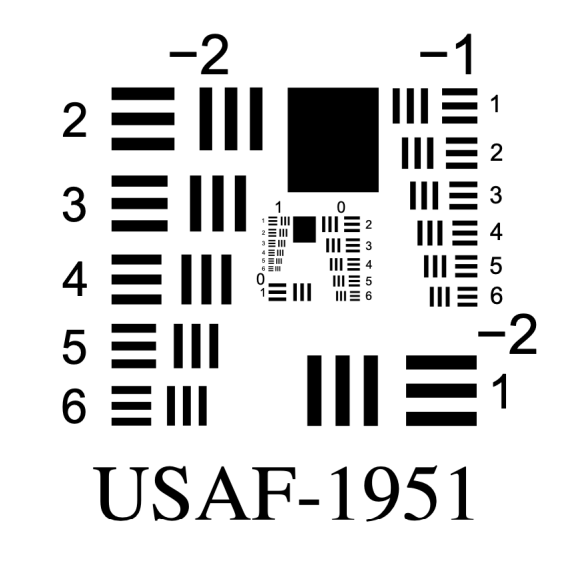
\includegraphics[width=.75\textwidth]{Images/AFTest.png}
    \caption{USAF Test Mask}
    \label{fig:Bill}
\end{figure}

\medskip \noindent
The lines in each column (group) and row (element) have a horizontal and vertical pattern with a calibrated width. See Figure \ref{fig:LW} for the line widths, given in micrometers. The limit of your spatial resolution occurs at the point where you start to lose contrast between the black and white lines. 

\begin{figure}[h!]
    \centering
    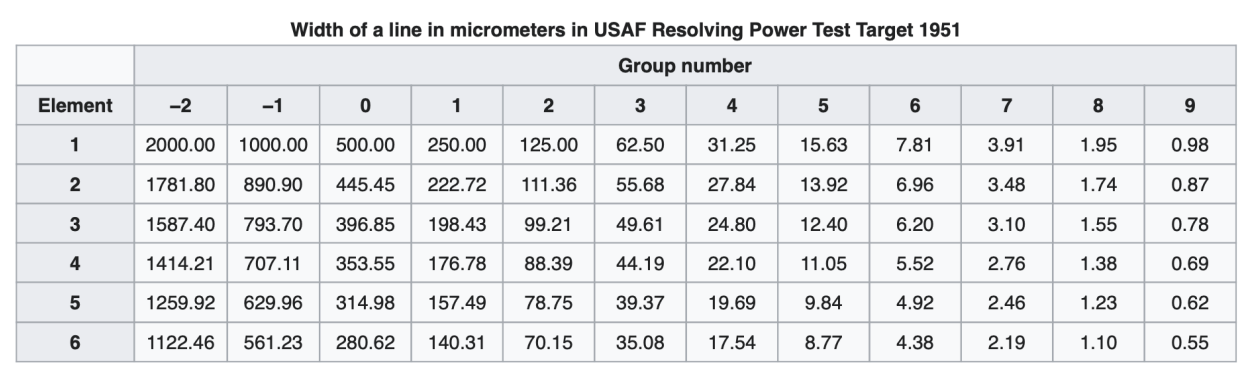
\includegraphics[width=.9\textwidth]{Images/LineWidths.png}
    \caption{Line Width Chart}
    \label{fig:LW}
\end{figure}

\medskip \noindent
We have setup two stations for this lab with the following:
\begin{enumerate}
    \item Binocular
    \item Larger diameter telescope with longer objective focal length
\end{enumerate}

\bigskip \noindent
On the far wall should be posted a USAF resolution test mask.

\medskip \noindent
16. For each binocular or telescope \textbf{[Record your results in a table your lab notebook]}:
\begin{enumerate}
    \item[A.] Distance to the target object (e.g. USAF 1951 test mask)
    \begin{enumerate}
    \item[-] Measure the distance between the telescope/binoculars and an object (e.g. object taped to a wall).
    \end{enumerate}
    \item[B.] Image orientation through the telescope: Note if the image is flipped/inverted or not.

    \item[C.] Field of View (FOV):
    \begin{enumerate}
    \item[-] Using a ruler, Determine the width of the field of view (FOV) through the binoculars or telescope in mm. Also do this for the two different eyepieces.
    \item[-] Use trigonometry to calculate approximate FOV angle in degrees.
    \end{enumerate}
    \item[D.] Angular resolution:
    \begin{enumerate}
    \item[-] What is the minimum line separation on the USAF Test Mask you can resolve with this instrument? Record this carefully using the group (column) and element (row) numbers. Try this with each eyepiece.
    \item[-] Convert these to an angular resolution in arcseconds (“).
    \end{enumerate}

\end{enumerate}

\pagebreak \noindent
\textbf{Additional Questions:}
\begin{enumerate}
\setcounter{enumi}{16}
    \item Based on the field of view values you measured above, which instrument should we use to observe the following objects (telescope, binoculars, microscope)? You’ll need to look up the full angular extent of these objects.
    \begin{itemize}
        \item Moon
        \item Andromeda Galaxy
        \item Mars
    \end{itemize}
\end{enumerate}


\section{Wrapping Things Up}
\noindent Please complete this section on your own.
\begin{enumerate}
\setcounter{enumi}{17}
    \item Do you have any feedback about this lab?
    
    \item Post one (or more!) remaining question(s) you have about exoplanets to the Ed Discussion board.

\end{enumerate}

\end{document}